\documentclass{beamer}
\usepackage{color}
\usepackage{bm}
\usepackage{graphicx}
\usepackage{hyperref}
\usepackage{listings}
\beamertemplatenavigationsymbolsempty
\definecolor{mygreen}{rgb}{0,0.6,0}
\definecolor{mymauve}{rgb}{0.58,0,0.82}
\lstset{ %
  backgroundcolor=\color{white},   % choose the background color; you must add \usepackage{color} or \usepackage{xcolor}
  basicstyle=\footnotesize,        % the size of the fonts that are used for the code
  commentstyle=\color{mygreen},    % comment style
  deletekeywords={...},            % if you want to delete keywords from the given language
  extendedchars=true,              % lets you use non-ASCII characters; for 8-bits encodings only, does not work with UTF-8
  frame=single,                    % adds a frame around the code
  keywordstyle=\color{blue},       % keyword style
  language=Python,                 % the language of the code
  rulecolor=\color{black},         % if not set, the frame-color may be changed on line-breaks within not-black text (e.g. comments (green here))
  showspaces=false,                % show spaces everywhere adding particular underscores; it overrides 'showstringspaces'
  showstringspaces=false,          % don't show spaces in strings
  stringstyle=\color{mymauve},     % string literal style
  title=\lstname                   % show the filename of files included with \lstinputlisting; also try caption instead of title
}
\hypersetup{
    colorlinks=true,
    urlcolor=blue
}

\graphicspath{ {./img/} {./charts/} }


\title{Django on AWS}
\author{Adam Johnson - me@adamj.eu}
\date{14 December 2015}

\begin{document}


\maketitle


\begin{frame}[fragile]\frametitle{What is AWS?}

    \begin{itemize}
        \item Amazon Web Services, the biggest cloud service provider
        \item Who is using, or has used, AWS? With Django?
    \end{itemize}

    \begin{center}
        
\includegraphics[width=10cm]{aws}
    \end{center}

\end{frame}


\begin{frame}[fragile]\frametitle{What is AWS?}

    \begin{center}
        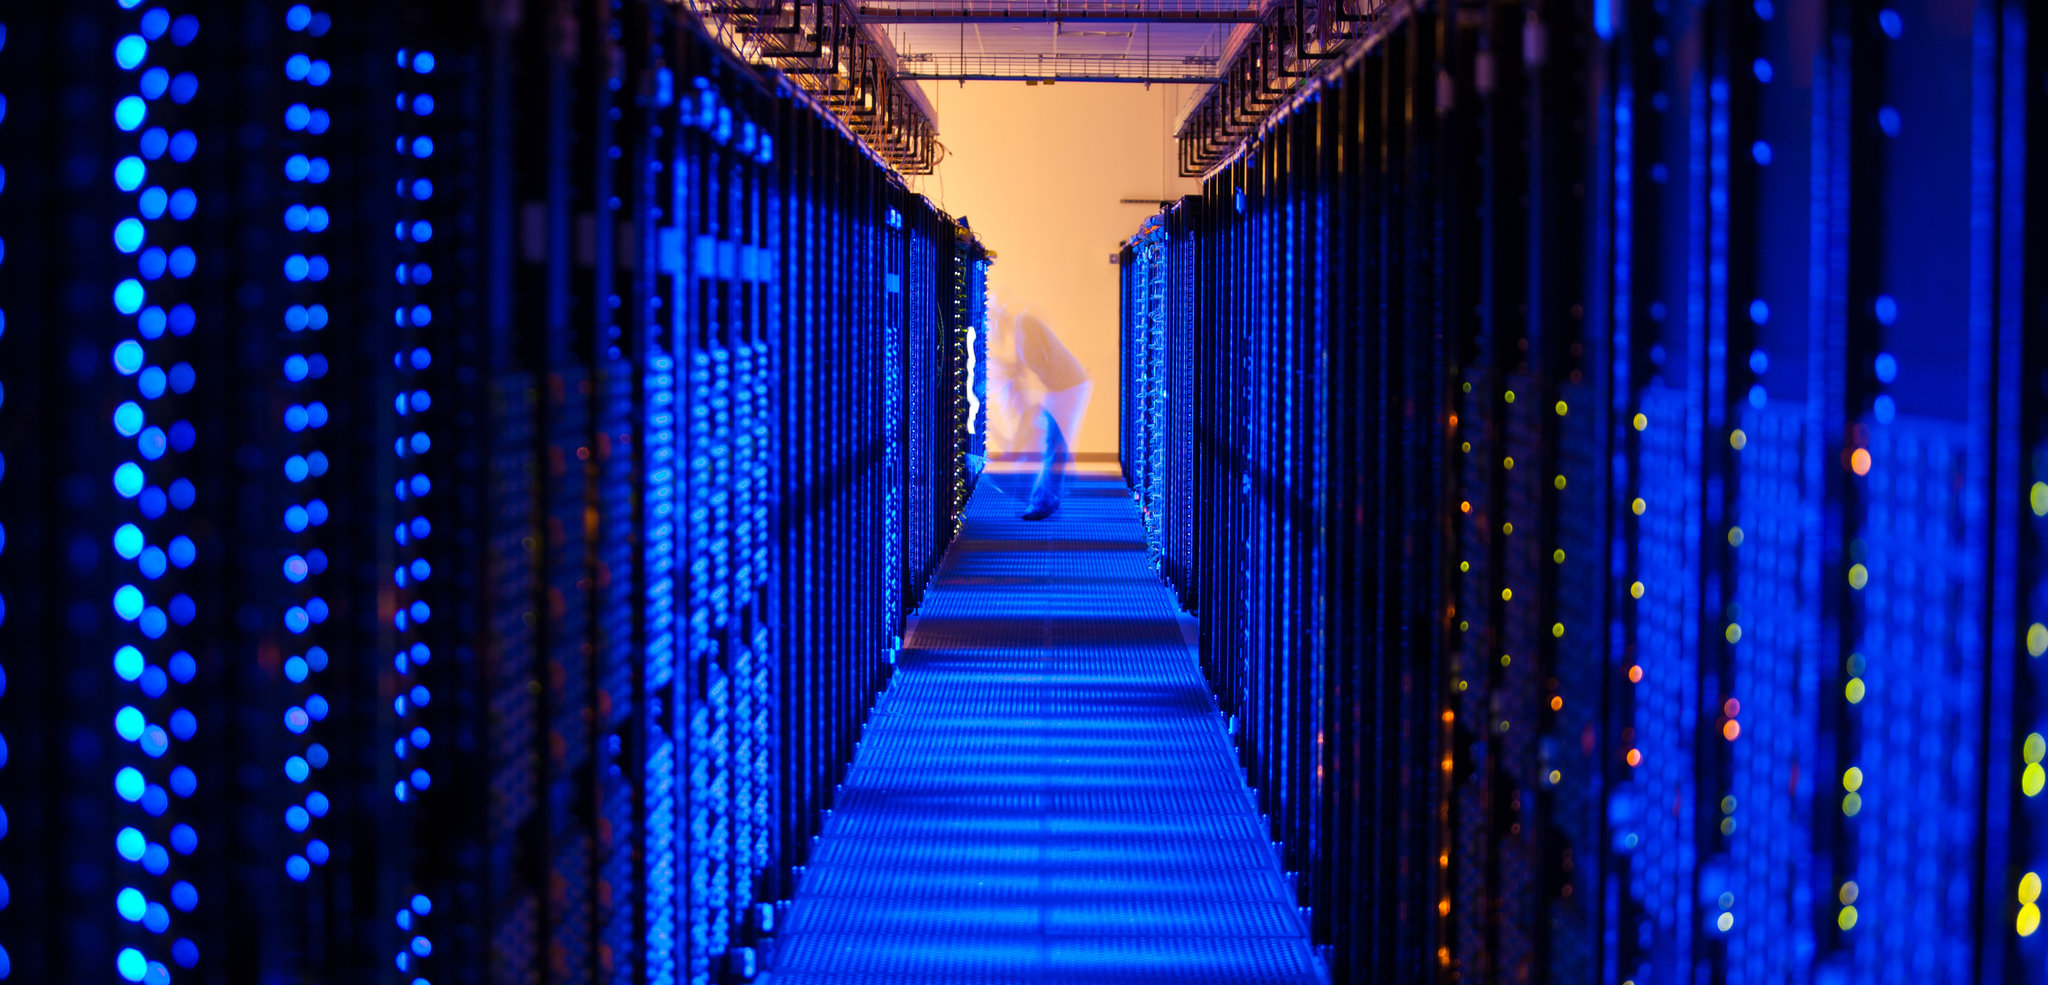
\includegraphics[width=10cm]{aws-dc}
    \end{center}

\end{frame}


\begin{frame}[fragile]\frametitle{Services}

    \begin{itemize}
        \item Hundreds of services!
        \item Compute, database, queueing, DNS, auditing, git repos, email, ...
        \item Some high level, some low level. Typically Django apps use more of the low level stuff.
    \end{itemize}

    \begin{center}
        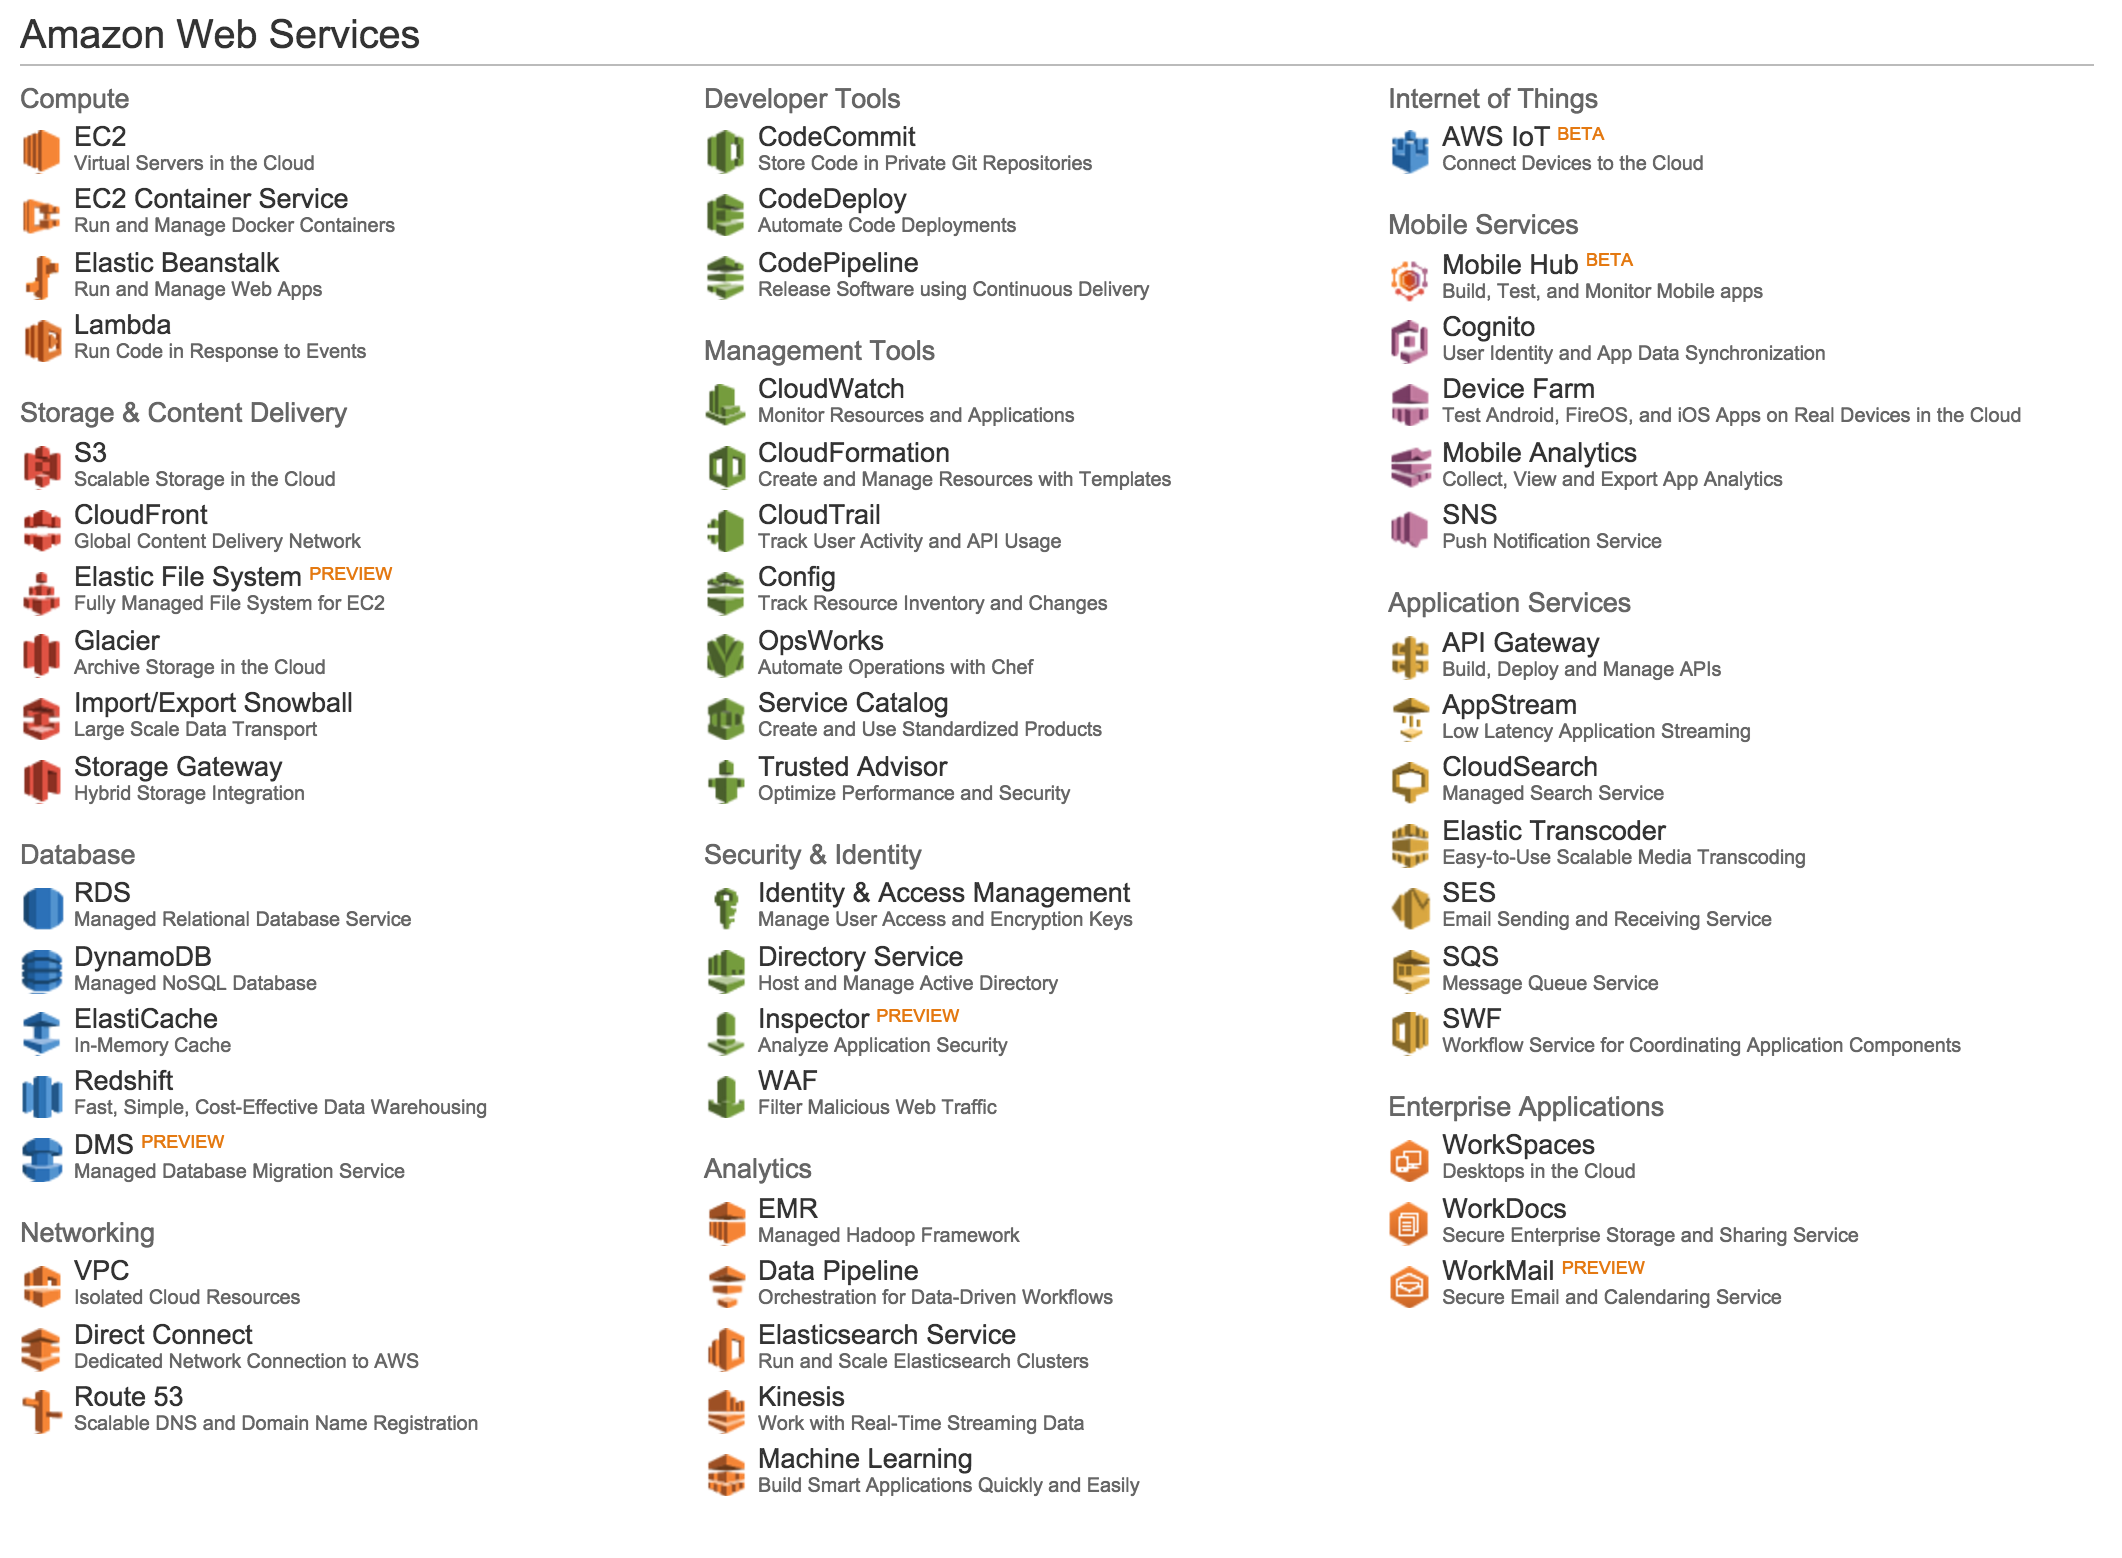
\includegraphics[width=8cm]{aws-services}
    \end{center}

\end{frame}


\begin{frame}[fragile]\frametitle{EC2}

    \begin{itemize}
        \item \textbf{Elastic Compute Cloud}
        \item Virtual servers, with a dizzying amount of options.
        \item Use in a Django app: web servers, task servers, and other services e.g. monitoring.
        \item Treat them as ephemeral - use automation so you can launch a new server within minutes. They aren't guaranteed to last forever.
    \end{itemize}

    \begin{center}
        
\includegraphics[width=3cm]{aws-ec2}
    \end{center}

\end{frame}


\begin{frame}[fragile]\frametitle{RDS}

    \begin{itemize}
        \item \textbf{Relational Database Service}
        \item Managed database servers - all the major Django DB's available: MariaDB, MS SQL, MySQL, Oracle, PostgreSQL.
        \item Important features: solid backups with easy restore, automated operations such as adding read-replicas, and redundancy.
        \item Don't run your database yourself on EC2 unless you have very specific requirements - hard to build the same robustness as RDS.
    \end{itemize}

    \begin{center}
        
\includegraphics[width=3cm]{aws-rds}
    \end{center}

\end{frame}


\begin{frame}[fragile]\frametitle{S3}

    \begin{itemize}
        \item \textbf{Simple Storage Service}
        \item Like a filesystem, but with unlimited storage and guaranteed high durability (99.999999999\%).
        \item Store things that don't go in the database - Django's static and media files.
        \item Storage backend \texttt{S3BotoStorage} from \texttt{django-storages-redux} makes it really easy.
    \end{itemize}

    \begin{center}
        
\includegraphics[width=3cm]{aws-s3}
    \end{center}

\end{frame}


\begin{frame}[fragile]\frametitle{S3 to the internet}

    \begin{itemize}
        \item S3 can serve direct to the internet itself, which often works, however it is not fully featured, e.g. it won't gzip assets if the client can use them.
        \item Easy to configure your webserver to sit in front of it though, e.g. \texttt{nginx}:
    \end{itemize}

    \begin{lstlisting}[basicstyle=\scriptsize]
location /static/ {
  proxy_hide_header x-amz-id-2;
  proxy_hide_header x-amz-request-id;
  expires max;
  proxy_pass https://s3-eu-west-1.amazonaws.com/my-bucket/;
}
    \end{lstlisting}

\end{frame}


\begin{frame}[fragile]\frametitle{Cloudfront}

    \begin{itemize}
        \item Content Delivery Network (CDN) - faster delivery of your content via private global network with "edges" that cache and serve to clients
        \item 54 locations worldwide - 3 in London!
        \item Makes your static assets faster
        \item Can also speed up your dynamic content - no caching, but private network still give a speed boost
    \end{itemize}

    \begin{center}
        
\includegraphics[width=3cm]{aws-cloudfront}
    \end{center}

\end{frame}


\begin{frame}[fragile]\frametitle{IAM}

    \begin{itemize}
        \item \textbf{Identity Access Management}
        \item Create users for your account, allow login with password or API key, grant granular permissions
        \item Some security hints:
        \begin{itemize}
            \item Never use your root account
            \item Activate Multi Factor Authentication on all accounts
            \item Use EC2 IAM Roles - permissions automatically granted to machine, no password required in your Django settings!
        \end{itemize}
    \end{itemize}

    \begin{center}
        
\includegraphics[width=3cm]{aws-iam}
    \end{center}

\end{frame}


\begin{frame}[fragile]\frametitle{YPlan on AWS}

    Pretty much as I've been discussing:

    \begin{itemize}
        \item MySQL on RDS
        \item Static and media assets in S3, served via Cloudfront and webservers
        \item Web and Celery on EC2: each build, we freeze an Amazon Machine Image (AMI) for each deployment using Ansible - all code, dependencies, etc. included. AMI deployed as multiple instances in several Autoscaling groups.
        \item Memcached in EC2 autoscaling group too - \textbf{Elasticache} became annoying
    \end{itemize}

\end{frame}


\begin{frame}[fragile]\frametitle{AWS vs other cloud providers}

    \begin{itemize}
        \item Most Cloud providers have equivalents of EC2 and S3 - in fact often API compatible.
        \item However can lack other services. AWS tend to build every little thing to attract all types of customers, however it makes things very complex.
        \item Might be a bit more \$ per CPU cycle, but imo the added value from services is worth it
    \end{itemize}

    \begin{center}
        
\includegraphics[width=7cm]{clouds}
    \end{center}

\end{frame}


\begin{frame}[fragile]\frametitle{Thank You}

    \begin{center}
        
\includegraphics[width=10cm]{cow-clouds}
    \end{center}

    \begin{itemize}
        \item My blog: \url{adamj.eu/tech/}
    \end{itemize}

\end{frame}


\end{document}
